%%%%%%%%%%%%%%%%%%%%%%%%%%%%%%%%%%%%%%%%%
% Stylish Article
% LaTeX Template
% Version 2.1 (1/10/15)
%
% This template has been downloaded from:
% http://www.LaTeXTemplates.com
%
% Original author:
% Mathias Legrand (legrand.mathias@gmail.com) 
% With extensive modifications by:
% Vel (vel@latextemplates.com)
%
% License:
% CC BY-NC-SA 3.0 (http://creativecommons.org/licenses/by-nc-sa/3.0/)
%
%%%%%%%%%%%%%%%%%%%%%%%%%%%%%%%%%%%%%%%%%

%----------------------------------------------------------------------------------------
%	PACKAGES AND OTHER DOCUMENT CONFIGURATIONS
%----------------------------------------------------------------------------------------

\documentclass[fleqn,10pt]{SelfArx} % Document font size and equations flushed left

\usepackage{subcaption}
\usepackage[english]{babel} % Specify a different language here - english by default
\usepackage{array,booktabs}% http://ctan.org/pkg/{array,booktabs}
\usepackage{lipsum} % Required to insert dummy text. To be removed otherwise
\usepackage[section]{placeins}
\usepackage{amsmath}
\newcolumntype{P}[1]{>{\centering\arraybackslash}p{#1}}
\newcolumntype{M}[1]{>{\centering\arraybackslash}m{#1}}
%----------------------------------------------------------------------------------------
%	COLUMNS
%----------------------------------------------------------------------------------------

\setlength{\columnsep}{0.55cm} % Distance between the two columns of text
\setlength{\fboxrule}{0.75pt} % Width of the border around the abstract

%----------------------------------------------------------------------------------------
%	COLORS
%----------------------------------------------------------------------------------------

\definecolor{color1}{RGB}{0,0,90} % Color of the article title and sections
\definecolor{color2}{RGB}{0,20,20} % Color of the boxes behind the abstract and headings

%----------------------------------------------------------------------------------------
%	HYPERLINKS
%----------------------------------------------------------------------------------------

\usepackage{hyperref} % Required for hyperlinks
\hypersetup{hidelinks,colorlinks,breaklinks=true,urlcolor=color2,citecolor=color1,linkcolor=color1,bookmarksopen=false,pdftitle={Title},pdfauthor={Author}}

%----------------------------------------------------------------------------------------
%	ARTICLE INFORMATION
%----------------------------------------------------------------------------------------

\JournalInfo{\today} % Journal information
\Archive{} % Additional notes (e.g. copyright, DOI, review/research article)

\PaperTitle{{\small ESE650 Project 4:} \\Simultaneous Localization and Mapping} % Article title

\Authors{Nischal K N\\nischal@seas.upenn.edu} % Authors
%\affiliation{\textsuperscript{1}\textit{Department of Biology, University of Examples, London, United Kingdom}} % Author affiliation
%\affiliation{\textsuperscript{2}\textit{Department of Chemistry, University of Examples, London, United Kingdom}} % Author affiliation
%\affiliation{*\textbf{Corresponding author}: john@smith.com} % Corresponding author

\Keywords{} % Keywords - if you don't want any simply remove all the text between the curly brackets
\newcommand{\keywordname}{Keywords} % Defines the keywords heading name

%----------------------------------------------------------------------------------------
%	ABSTRACT
%----------------------------------------------------------------------------------------

\Abstract{Simultaneous Localization and Mapping(SLAM) is a problem of locating the position of an object in an unknown environment and keep track of it as it moves in that environment. It also involves generation of a map of the surroundings. In this project we use data from a LiDAR range sensor to generate the map of the environment in which a humanoid robot, THOR is moving in. Also a texture map of the ground is generated from the RGBD data provided by a kinect camera. The mapping is achieved using Monte Carlo Localization.}

%----------------------------------------------------------------------------------------

\begin{document}

\flushbottom % Makes all text pages the same height

\maketitle % Print the title and abstract box

\tableofcontents % Print the contents section

\thispagestyle{empty} % Removes page numbering from the first page

%----------------------------------------------------------------------------------------
%	ARTICLE CONTENTS
%----------------------------------------------------------------------------------------
\section{Introduction}
In this project we use the distances measured by a 2D laser range finder, use the odometry given by the kinematic model of the THOR and apply a particle filter with a Gaussian noise to localize as well as map the position of the robot in the environment it is moving in. The different data used and how they are accessed is explained in Section \ref{sec:pprocessing}. Section \ref{sec:algo} explains the various steps followed to perform SLAM. Section \ref{sec:param} explains the various tunable parameters use in the code and their values. The algorithm used to create the texture map is explained in Section \ref{sec:tm}. Finally the experiments and results are documented in Section \ref{sec:results}.

\section{Dataset}
\label{sec:pprocessing}
The dataset consists of data from lidar, kinect sensor, imu, joint encoders and kinematic model of THOR. The required data that was extracted and stored in a new file to simplify the process. This makes it easier to access the required data and also drastically reduces the dataset size preventing system overload. The script reFormatData.m performs this cleaning up. The following were the data extracted.
\begin{enumerate}
\item 2D lidar scans from an hokuyo 30lx LiDAR captured at a rate of 40Hz, with a maximum range of 30m and a $270^o$ view. The corresponding message time stamps are also recorded. 
\item joint angles of neck and head indicating the yaw and pitch of the head with time stamps.
\item pose estimation from the kinematic model of THOR.
\item RGB and Depth images from the kinect camera along with timestamps.
\end{enumerate}

\section{Algorithm}
\label{sec:algo}
The SLAM uses Monte Carlo localization with additional processing to remove ground and roof hits and skew correction due to tilt of the head. The basic flow of steps followed is shown in Fig. \ref{fig:algo}. Each of these steps are explained in the respective sections.

\begin{figure}[hbtp]
\centering
\includegraphics[scale=0.45]{slam.png}
\caption{Algorithm flowchart}
\label{fig:algo}
\end{figure}

\begin{figure*}
    \centering
    \begin{subfigure}[t]{0.3\textwidth}
        \centering
        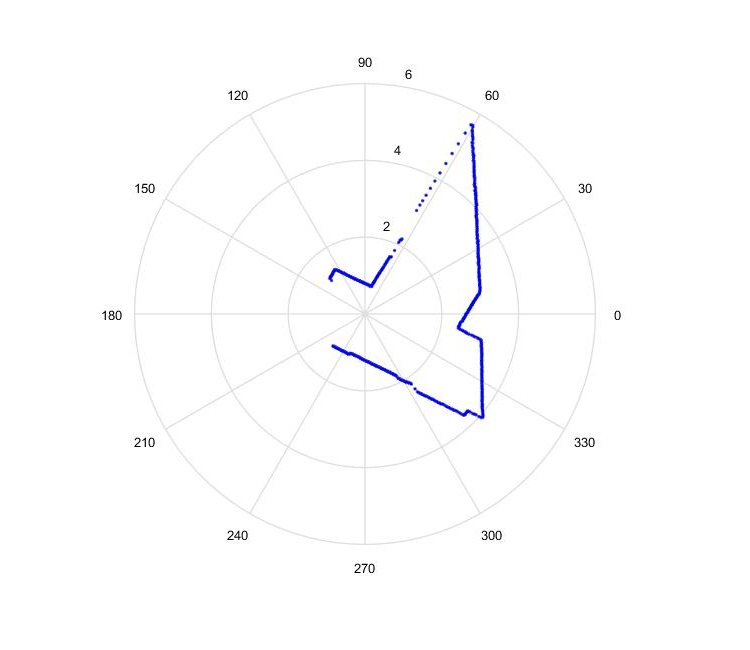
\includegraphics[scale = 0.3]{raw.jpg}
        \caption{Raw lidar scan}
    \end{subfigure}%
    ~ 
    \begin{subfigure}[t]{0.3\textwidth}
        \centering
        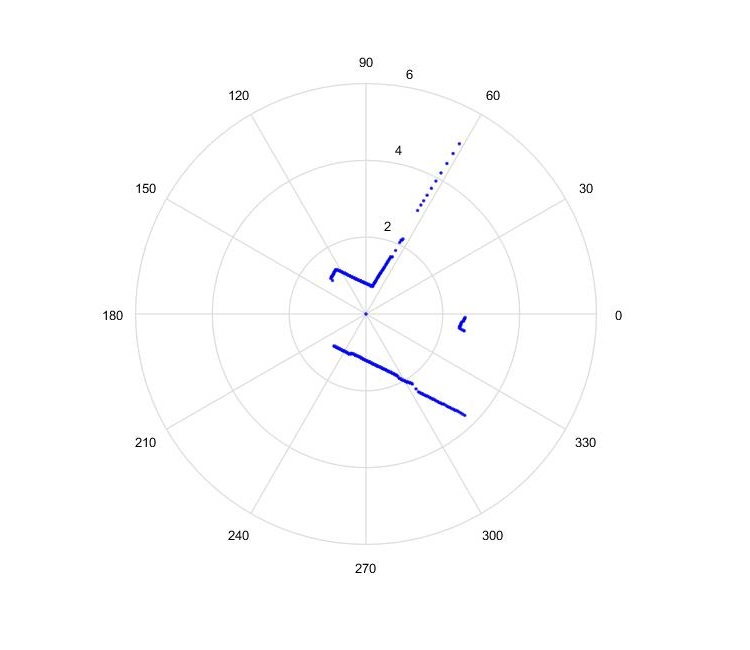
\includegraphics[scale = 0.3]{gr.jpg}
        \caption{Ground Removal}
    \end{subfigure}
    ~
    \begin{subfigure}[t]{0.3\textwidth}
        \centering
        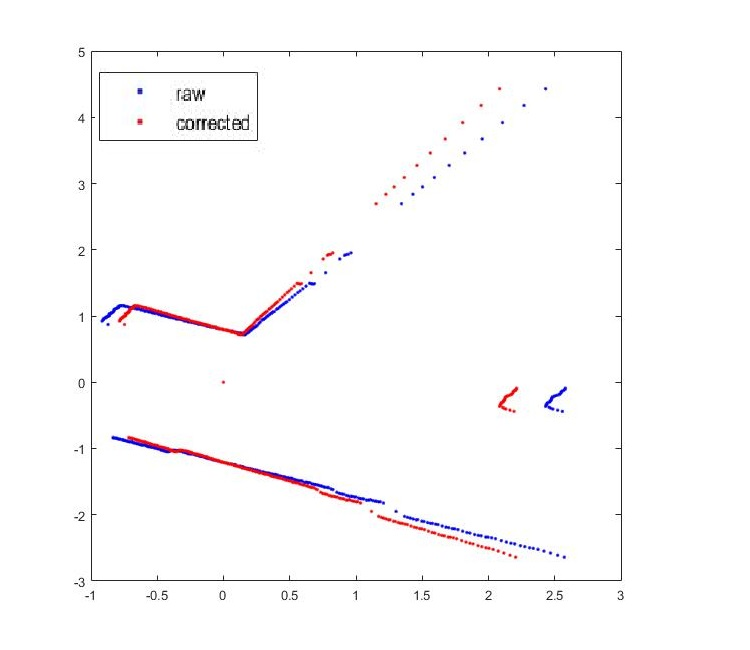
\includegraphics[scale = 0.3]{skew.jpg}
        \caption{Skew correction}
    \end{subfigure}
    \caption{Ground hit removal}
    \label{fig:gr}
\end{figure*}

\subsection{Ground Removal}
\label{subsec:ground}
The LiDAR is mounted on head that pitches up and down. This causes the LiDAR to pick up ground hits and detects them as walls. If these are not accounted for, then false walls may be recorded whenever the head pitches down or up. This removal was done by computing the following equation for each datapoint of LiDAR.
\begin{align*}
R \times sin(\theta) \times cos(\alpha) > H_{corrected} \\
\intertext{If this condition was satisfied, then the scan was removed, else the scan was retained. $H_{corrected}$ was the recalculated height considering the tilt of the head}
H_{corrected} = H_{actual} - 0.15 \times cos(\theta) \\
\end{align*}
Where $\theta$ was the pitch of the head and $\alpha$ was the angle of the scan between $-135^o$ to $135^o$. R is the distance measured by the LiDAR. The result of using the raw scan and $Rsin\theta cos\alpha$ is shown in fig. \ref{fig:gr}.

Additionally a skew correction of the LiDAR scans are performed to compensate for the head angle. This is performed using
\begin{align*}
R_{new} = R \times cos\theta
\end{align*}
This can be seen in \ref{fig:gr}c. The red is corrected scan and blue is the raw scan

\subsection{Initialization}
\label{subsec:init}
To initialize the SLAM algorithm, first the time stamps of LiDAR and joints are synced. Then a global map of a fixed dimension and resolution is initialized with 0 indicating unexplored area. Then the first scan is subjected to ground and skew removal. Then is placed on the center of the map by increasing the value of those cells of the global map where walls are assumed to be present by a logodd\_occ value, and decreasing the value of the cells where free space is detected by logodd\_free value. Also many parameters described in \ref{sec:param} are initialized here.

\subsection{Fixing Odometry}
\label{subsec:odom}
The odometry provided by the kinematic model of THOR is not in the same global frame of reference as our map. Hence it has to be explicitly computed by measuring the change in state between local frames. The following steps were performed.
\begin{enumerate}
\item Compute delta increment in wrong global frame
\begin{align*}
{[dx dy d\theta]}_{wrong} = {pose}_{cur}-{pose}_{prev}
\end{align*}
\item Convert to local frame
\begin{align*}
{yaw}_{wrong} =&\;  {pose}_{\theta prev} \\
{[dx dy]}_{local} =&\; 
\begin{bmatrix}
cos({yaw}_{wrong}) & sin({yaw}_{wrong}) \\
-sin({yaw}_{wrong}) & cos({yaw}_{wrong}) \\
\end{bmatrix} \\
&\; \times {[dx dy]}_{wrong} \\
{d\theta}_{local} =&\; {d\theta}_{wrong}
\end{align*}
\item Convert it to right global frame
\begin{align*}
{[dx dy]}_{global}=&\;
\begin{bmatrix}
cos(yaw) & -sin(yaw) \\
sin(yaw) & cos(yaw) \\
\end{bmatrix} \\
&\; \times {[dx dy]}_{local} \\
{d\theta}_{global} =&\; {d\theta}_{local } \\ 
x =&\; x+{dx}_{global} \\
y =&\; y+{dy}_{global} \\
\theta =&\; \theta+{d\theta}_{global} \\
\end{align*}
\end{enumerate}
x,y and theta is the new corrected global odometry that can be used for motion update of particles.

\subsection{Particle filter}
\label{subsec:pf}
A fixed number of particles were used. For each particle, a motion update was performed with a different noise parameter to the corrected global odometry. This resulted in n different orientations and position of LiDAR scans to be correlated with the global map. The noise parameters choosen are mentions in \ref{sec:param}.

\subsection{Correlation}
For this project, both map\_correlation mex file and corr2 matlab function was experimented. It was seen that both of them yield a similar result but corr2 being very slow compared to the mex file. The inputs to the mex file was positive version of the global logodds map. The negative values were reduced to zero and only the positive values were retained. The lidar scans passed to this fucntion were corrected for ground hit removal and skew correction. The correlation scores for each particle was recorded. It was multiplied with the weight of each particle and then normalized. The pose of the particle with the highest weight was chosen as the pose of the robot for that frame. This pose was used to update the global map by increasing and decreasing the logodd\_occ and logodd\_free values for walls and free space respectively. An upper and lower bound for logodd values were maintained.

\subsection{Re-sampling}
When ever the majority of weight of the particles were accumulated within a few particles, the particles were re-sampled based on the current weight. More particles were chosen from the particle with more weight and vice-a-verse. A random sampling was performed. Due to high number of particles used, there was no difference between the performance of random sampling and low variance sampling.

\section{Selecting Parameters}
\label{sec:param}
A number of parameters were used in the code that were tunable, the most prominent one that affected the performance were the motion update noise parameters, logodd saturation values and number of particles. The various parameters values used were
\begin{enumerate}
\item \textbf{No of Particles: 100}, less particles performed well then the motion was relatively straight like in dataset 2 and 1. But failed when there were turns.
\item \textbf{Number of Effective Particles: 40}
\item \textbf{Motion noise: 10cm(x\&y), $5^o$(theta)}, lower noise increases the trust on odometry and increasing it decreases the performance as particles are scattered over a wide area resulting in the need to increase the number of particles which in turn increases computation.
\item \textbf{logodd\_occ = 2.5 and logodd\_free = 0.625}, this is because the the datapoints of walls are far less compared to the free space data points.
\item \textbf{Map saturation threshold: 100 and -100}
\item \textbf{Map resolution: 5cm} Increasing the resolution increases the computation time but also improves the map quality.
\end{enumerate}

\section{Texture map}
\label{sec:tm}
Once the map was generated by SLAM, the kinect's RGBD data was used to generate the floor texture of the the map.

\begin{figure}[htbp]
\centering
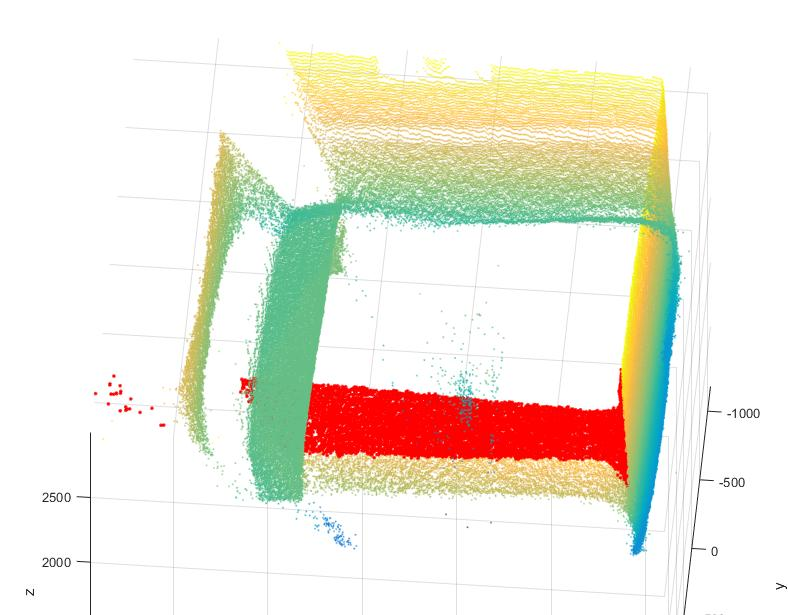
\includegraphics[scale=0.3]{pc.jpg}
\caption{Point Cloud with ground detected in red}
\label{fig:pc}
\end{figure}

\begin{figure}[htbp]
\centering
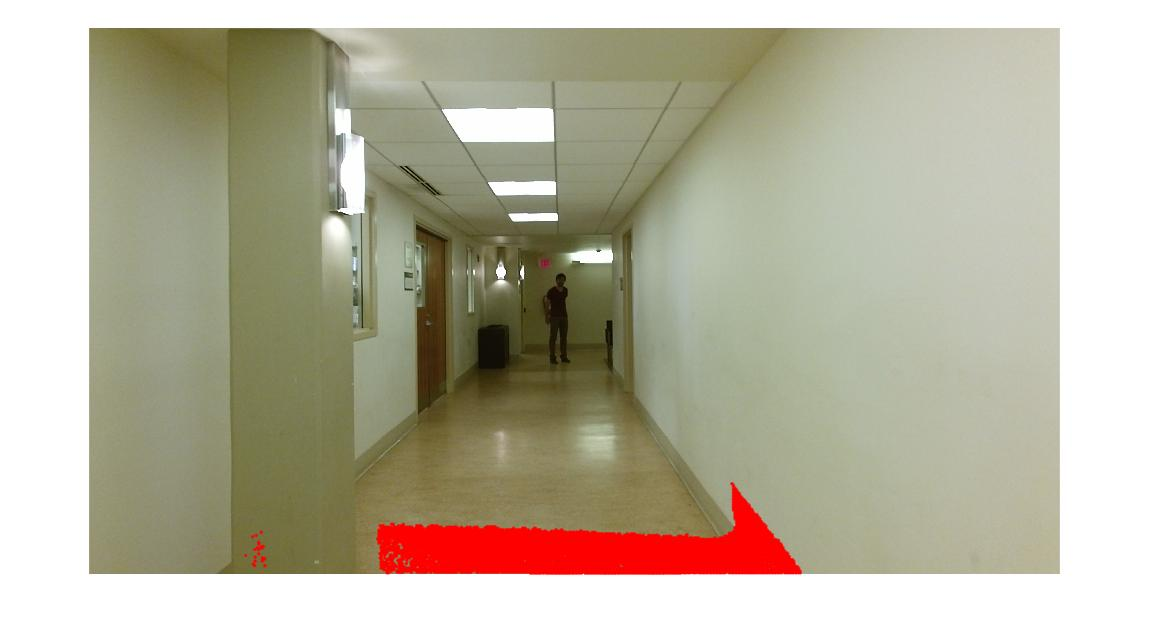
\includegraphics[scale=0.2]{rgb.jpg}
\caption{RGB image with detected ground points}
\label{fig:rgb}
\end{figure}

Following were the steps followed
\begin{enumerate}
\item The depth data, z were thresholded between 500 to 3000, the usable range of kinect data.
\item The depth image was projected to a 3D point in space generating a 3D point cloud as shown in fig. \ref{fig:pc} using
\begin{align*}
x = \frac{u \times z}{fc},  y = \frac{v \times z}{fc}
\end{align*}
where u and v are pixel coordinates, z is the depth and fc is the focal length.
\item The ground plane was detected from the point cloud by determining the points that lie on the plane satisfied by the equation
\begin{align*}
a_0x+a_1y+a_2z+a_3 <&\; \epsilon
\intertext{where $a_0$, $a_1$, $a_2$ and $a_3$ are 0,-1,0 and h. $\epsilon$ is the threshold. The head pitch $\theta$ is also accounted for using}
\begin{bmatrix}
a'_0 \\ a'_1 \\ a'_2 \\
\end{bmatrix} = 
\begin{bmatrix}
1 & 0 & 0 \\
0 & cos\theta & -sin\theta \\
0 & sin\theta & cos\theta \\
\end{bmatrix} \times&\;
\begin{bmatrix}
0 \\ -1 \\ 0 \\
\end{bmatrix}
\end{align*}
\item The depth coordinates are transformed into RGB coordinates using ${rgb}_{x,y,z} = R \times {depth}_{x,y,z} + T$
\item The points are projected back onto RGB image using shown in fig. \ref{fig:rgb}
\begin{align*}
u = \frac{fc \times x}{z}, v = \frac{fc \times y}{z}
\end{align*}
\item The ground points are also converted to LIDAR frame using, (R and T between lidar and kinect is ignored)
\begin{align*}
{LiDAR}_{x,y,z} = 
\begin{bmatrix}
0 & 0 & 1 \\
-1 & 0 & 0 \\
0 & -1 & 0 \\
\end{bmatrix}
\times {depth}_{x,y,z}
\end{align*}
\item These points are transformed with the pose of the best particle and then corresponding RGB pixel values are copied to the global map.
\end{enumerate}

\section{Experiments and Results}
\label{sec:results}
The algorithm was ran on 4 training datasets and also on the testing set. The output was consistent with the actual corridors. They are shown in fig. \ref{fig:train0} to fig. \ref{fig:test}. 

The video of color and RGB map generation for test set is present at

Grayscale map: \textbf{\hyperref[https://youtu.be/ykQvQrcE3Xk]{https://youtu.be/ykQvQrcE3Xk}}
Texture map: \textbf{\hyperref[https://youtu.be/SuZ3QX5SUrM]{https://youtu.be/SuZ3QX5SUrM}}

\begin{figure*}
    \centering
    \begin{subfigure}[t]{0.5\textwidth}
        \centering
        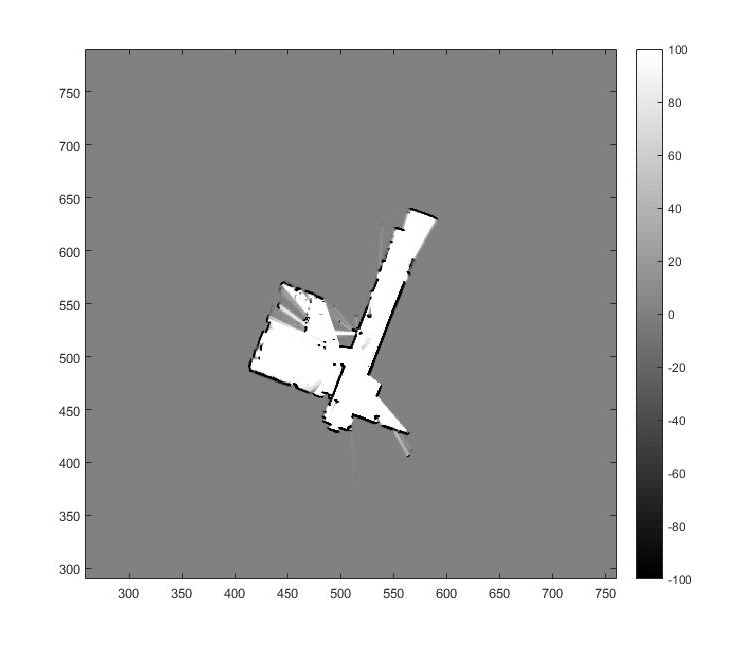
\includegraphics[scale = 0.5]{set0_map.jpg}
        \caption{gray scale Map}
    \end{subfigure}%
    ~ 
    \begin{subfigure}[t]{0.5\textwidth}
        \centering
        
\includegraphics[scale = 0.5]{set0_tm.jpg}
        \caption{Floor Texture}
    \end{subfigure}
    \caption{Training Dataset 0}
    \label{fig:train0}
\end{figure*}

\begin{figure*}
    \centering
    \begin{subfigure}[t]{0.5\textwidth}
        \centering
        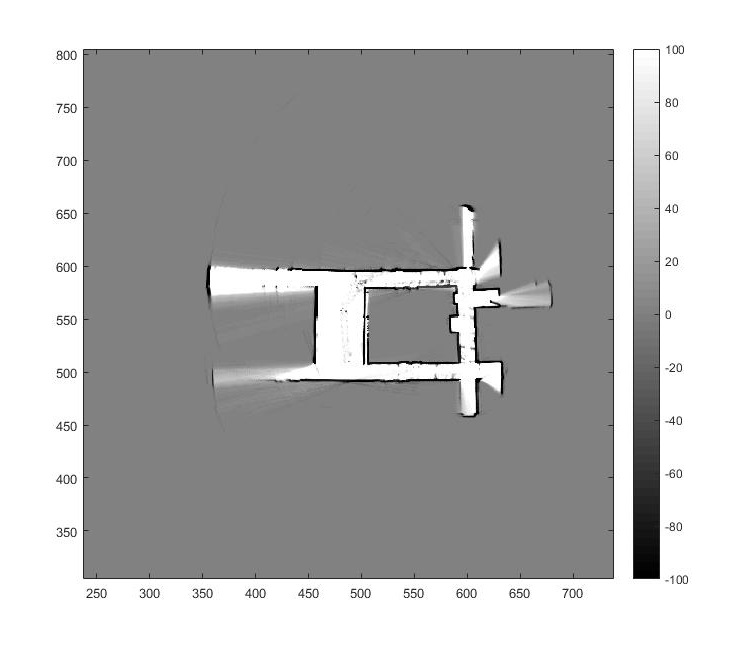
\includegraphics[scale = 0.5]{set1_map.jpg}
        \caption{gray scale map for training dataset 1}
    \end{subfigure}%
    ~ 
    \begin{subfigure}[t]{0.5\textwidth}
        \centering
        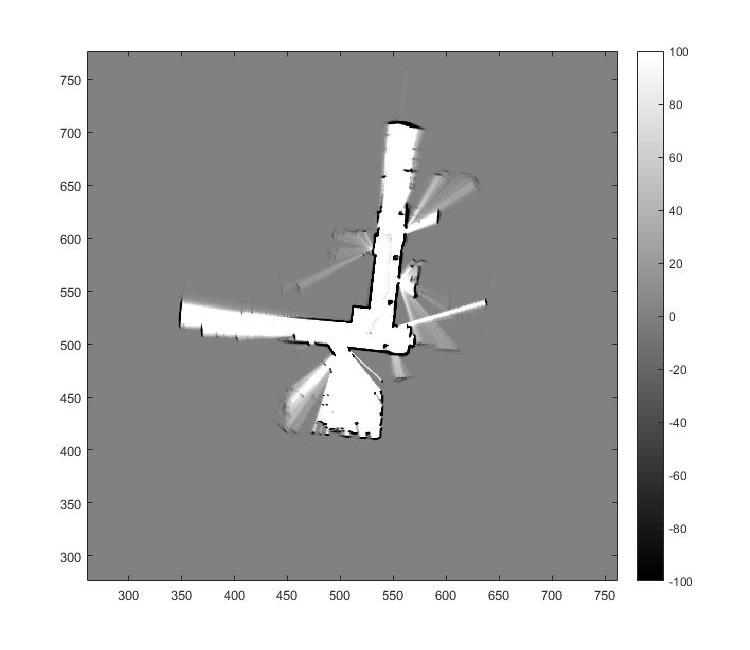
\includegraphics[scale = 0.5]{set2_map.jpg}
        \caption{gray scale map for training dataset 2}
    \end{subfigure}
    \caption{Training Dataset 1 and 2}
    \label{fig:train12}
\end{figure*}

\begin{figure*}
    \centering
    \begin{subfigure}[t]{0.5\textwidth}
        \centering
        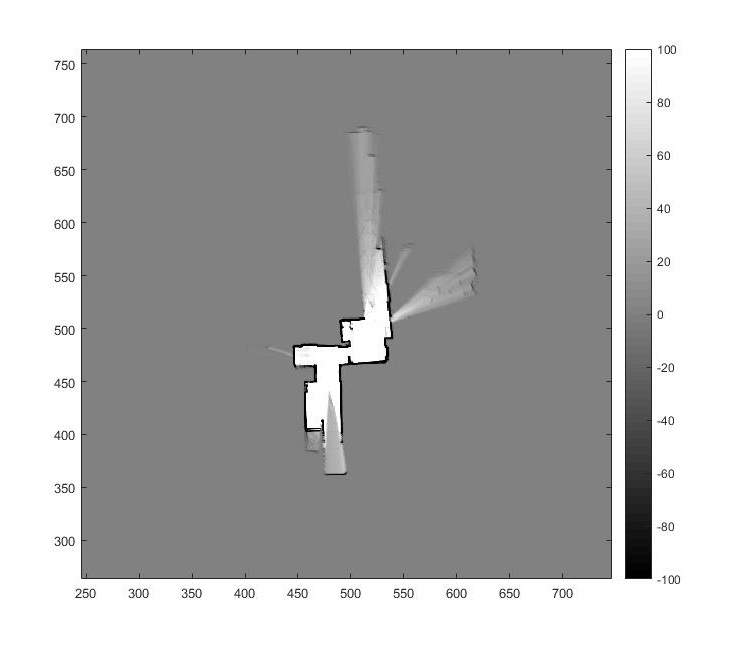
\includegraphics[scale = 0.5]{set3_map.jpg}
        \caption{gray scale Map}
    \end{subfigure}%
    ~ 
    \begin{subfigure}[t]{0.5\textwidth}
        \centering
        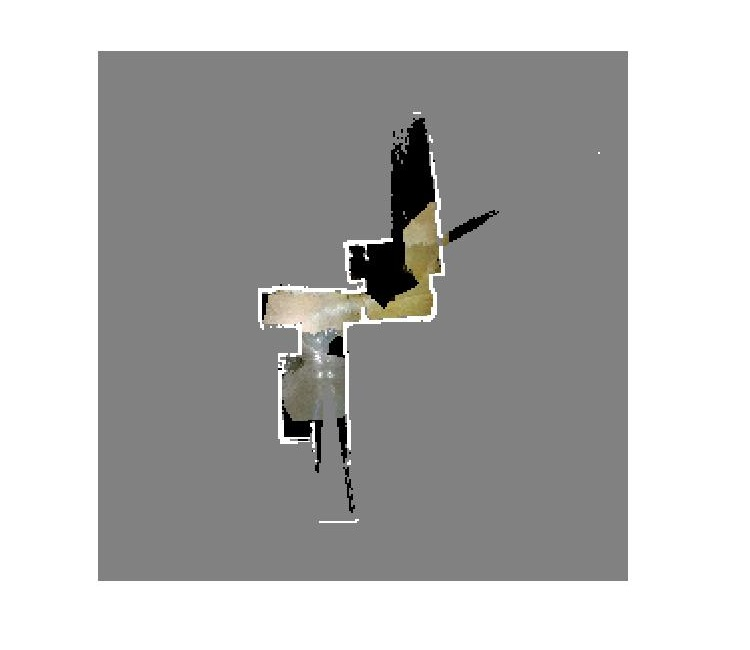
\includegraphics[scale = 0.5]{set3_tm.jpg}
        \caption{Floor Texture}
    \end{subfigure}
    \caption{Training Dataset 3}
    \label{fig:train3}
\end{figure*}

\begin{figure*}
    \centering
    \begin{subfigure}[t]{0.5\textwidth}
        \centering
        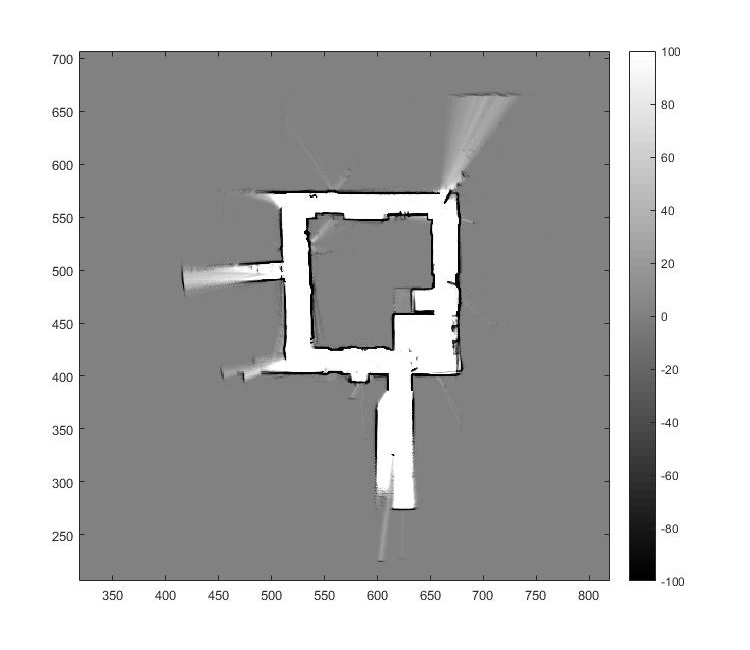
\includegraphics[scale = 0.5]{test_map.jpg}
        \caption{gray scale Map}
    \end{subfigure}%
    ~ 
    \begin{subfigure}[t]{0.5\textwidth}
        \centering
        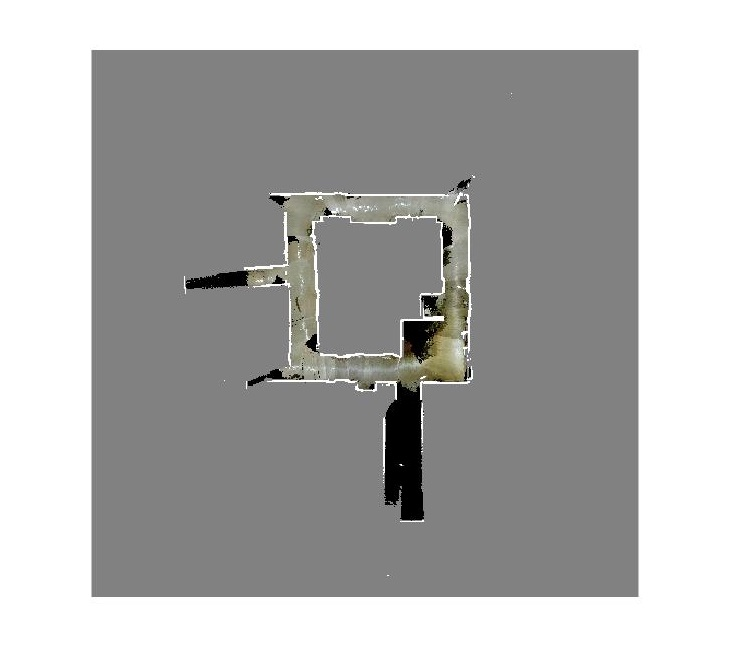
\includegraphics[scale = 0.5]{test_tm.jpg}
        \caption{Floor Texture}
    \end{subfigure}
    \caption{Test Dataset}
    \label{fig:test}
\end{figure*}

%\begin{thebibliography}{9}

%\end{thebibliography}

%----------------------------------------------------------------------------------------
%	REFERENCE LIST
%----------------------------------------------------------------------------------------
%\phantomsection
%\bibliographystyle{unsrt}
%\bibliography{sample}

%---------------------------------------------------------------------------------------- 

\end{document}

%% Convergence graph
%% State transition matrixes
%% Cross validation matrix